%%% The main file. It contains definitions of basic parameters and includes all other parts.

% Meta-data of your thesis (please edit)
\input metadata.tex

% Generate metadata in XMP format for use by the pdfx package
\input xmp.tex

%% Settings for single-side (simplex) printing
% Margins: left 40mm, right 25mm, top and bottom 25mm
% (but beware, LaTeX adds 1in implicitly)
%\documentclass[12pt,a4paper]{report}
%\setlength\textwidth{145mm}
%\setlength\textheight{247mm}
%\setlength\oddsidemargin{15mm}
%\setlength\evensidemargin{15mm}
%\setlength\topmargin{0mm}
%\setlength\headsep{0mm}
%\setlength\headheight{0mm}
% \openright makes the following text appear on a right-hand page
%\let\openright=\clearpage

%% Settings for two-sided (duplex) printing
 \documentclass[12pt,a4paper,twoside,openright]{report}
 \setlength\textwidth{145mm}
 \setlength\textheight{247mm}
 \setlength\oddsidemargin{14.2mm}
 \setlength\evensidemargin{0mm}
 \setlength\topmargin{0mm}
 \setlength\headsep{0mm}
 \setlength\headheight{0mm}
 \let\openright=\cleardoublepage

%% Generate PDF/A-2u
\usepackage[a-2u]{pdfx}

%% Prefer Latin Modern fonts
\usepackage{lmodern}

% If we are not using LuaTeX, we need to set up character encoding:
\usepackage{iftex}
\ifpdftex
\usepackage[utf8]{inputenc}
\usepackage[T1]{fontenc}
\usepackage{textcomp}
\fi

%% Further useful packages (included in most LaTeX distributions)
\usepackage{amsmath,amssymb}         % extensions for typesetting of math
\usepackage{amsfonts}                % math fonts
\usepackage{amsthm}                  % theorems, definitions, etc.
\usepackage{bm}                      % boldface symbols (\bm)
\usepackage{booktabs}                % improved horizontal lines in tables
\usepackage{caption}                 % custom captions of floating objects (MY OPTION)
\usepackage{dcolumn}                 % improved alignment of table columns
\usepackage{floatrow}                % custom float environments
\usepackage{graphicx}                % embedding of pictures
\usepackage{indentfirst}             % indent the first paragraph of a chapter
\usepackage[nopatch=item]{microtype} % micro-typographic refinement
\usepackage{paralist}                % improved enumerate and itemize
\usepackage[nottoc]{tocbibind}       % makes sure that bibliography and the lists
									 % of figures/tables are included in the table
									 % of contents
\usepackage{xcolor}                  % typesetting in color

% The hyperref package for clickable links in PDF and also for storing
% metadata to PDF (including the table of contents).
% Most settings are pre-set by the pdfx package.
\hypersetup{unicode}
\hypersetup{breaklinks=true}
%%% if needed (old?)
%\hypersetup{
%	colorlinks=true,
%	allcolors=black,  % Sets all other links (non-URLs) to black/unstyled
%	urlbordercolor=blue,
%	pdfborder={0 0 1},
%	urlcolor=blue
%}

% Packages for computer science theses
\usepackage{algpseudocode}  % part of algorithmicx package
\usepackage{algorithm}
\usepackage{fancyvrb}       % improved verbatim environment
\usepackage{listings}       % pretty-printer of source code

% You might want to use cleveref for references --> MY OPTION
\usepackage[capitalise,nameinlink]{cleveref}
\creflabelformat{equation}{#2\textup{#1}#3}
\crefname{equation}{Eq.}{Eqs.}
\Crefname{equation}{Eq.}{Eqs.}
\crefname{section}{Sec.}{Secs.}
\Crefname{section}{Sec.}{Secs.}
\crefname{table}{Tab.}{Tabs.}
\Crefname{table}{Tab.}{Tabs.}

%%% MY OPTIONS %%%
\usepackage{float}			         % force picture placement
\usepackage{xspace}			         % space insertion in macros
\usepackage{textcomp}
\usepackage{siunitx}
\usepackage{physics}
\sisetup{
	per-mode=symbol,
	range-phrase = -,
	range-units = single,
	product-units = power
	}
\AtBeginDocument{\RenewCommandCopy\qty\SI}
\ExplSyntaxOn
\msg_redirect_name:nnn { siunitx } { physics-pkg } { none }
\ExplSyntaxOff
\show\qty
\usepackage{subcaption}
\captionsetup[subfigure]{font=footnotesize}
\usepackage{enumitem}
\usepackage[warnundef]{jabbrv}
\usepackage{acronym}
%%% MY OPTIONS (end) %%%

%%% OLD
%%% \usepackage{lineno}	% line numbering
%%% \linenumbers
%%% \usepackage{hyperref}   % references to sections

% Set up formatting of bibliography (references to literature)
% Details can be adjusted in macros.tex.
%
% BEWARE: Different fields of research and different university departments
% have their own customs regarding bibliography. Consult the bibliography
% format with your supervisor.
%
% The basic format according to the ISO 690 standard with numbered references
\usepackage[natbib,style=iso-numeric,sorting=none,backend=biber]{biblatex}
% ISO 690 with alphanumeric references (abbreviations of authors' names)
%\usepackage[natbib,style=iso-alphabetic]{biblatex}
% ISO 690 with references Author (year)
%\usepackage[natbib,style=iso-authoryear]{biblatex}
%
% Some fields of research prefer a simple format with numbered references
% (sorting=none tells that bibliography should be listed in citation order)
%\usepackage[natbib,style=numeric,sorting=none]{biblatex}
% Numbered references, but [1,2,3,4,5] is compressed to [1-5]
%\usepackage[natbib,style=numeric-comp,sorting=none]{biblatex}
% A simple format with alphanumeric references:
%\usepackage[natbib,style=alphabetic]{biblatex}

% Load the file with bibliography entries
\addbibresource{bibliography.bib}

% Definitions of macros (see description inside)
%%% This file contains definitions of various useful macros and environments %%%
%%% Please add more macros here instead of cluttering other files with them. %%%

%%% Minor tweaks of style

% These macros employ a little dirty trick to convince LaTeX to typeset
% chapter headings sanely, without lots of empty space above them.
% Feel free to ignore.
\makeatletter
\def\@makechapterhead#1{
	{\parindent \z@ \raggedright \normalfont
		\Huge\bfseries \thechapter. #1
		\par\nobreak
		\vskip 20\p@
}}
\def\@makeschapterhead#1{
	{\parindent \z@ \raggedright \normalfont
		\Huge\bfseries #1
		\par\nobreak
		\vskip 20\p@
}}
\makeatother

% This macro defines a chapter, which is not numbered, but is included
% in the table of contents.
\def\chapwithtoc#1{
	\chapter*{#1}
	\addcontentsline{toc}{chapter}{#1}
}

% Draw black "slugs" whenever a line overflows, so that we can spot it easily.
\overfullrule=1mm

%%% Macros for definitions, theorems, claims, examples, ... (requires amsthm package)

\theoremstyle{plain}
\newtheorem{thm}{Theorem}
%\newtheorem{lemma}[thm]{Lemma}
\newtheorem{claim}[thm]{Claim}

\theoremstyle{plain}
\newtheorem{defn}{Definition}

\theoremstyle{remark}
\newtheorem*{cor}{Corollary}
\newtheorem*{rem}{Remark}
\newtheorem*{example}{Example}

%%% An environment for proofs

\newenvironment{myproof}{
	\par\medskip\noindent
	\textit{Proof}.
}{
	\newline
	\rightline{$\qedsymbol$}
}

%%% An environment for typesetting of program code and input/output
%%% of programs. (Requires the fancyvrb package -- fancy verbatim.)

\DefineVerbatimEnvironment{code}{Verbatim}{fontsize=\small, frame=single}

%%% The field of all real and natural numbers
\newcommand{\R}{\mathbb{R}}
\newcommand{\N}{\mathbb{N}}

%%% Useful operators for statistics and probability
\DeclareMathOperator{\pr}{\textsf{P}}
\DeclareMathOperator{\E}{\textsf{E}\,}
%\DeclareMathOperator{\var}{\textrm{var}}
\DeclareMathOperator{\sd}{\textrm{sd}}

%%% Transposition of a vector/matrix
\newcommand{\T}[1]{#1^\top}

%%% Various math goodies
\newcommand{\goto}{\rightarrow}
\newcommand{\gotop}{\stackrel{P}{\longrightarrow}}
\newcommand{\maon}[1]{o(n^{#1})}
%\newcommand{\abs}[1]{\left|{#1}\right|}
\newcommand{\dint}{\int_0^\tau\!\!\int_0^\tau}
\newcommand{\isqr}[1]{\frac{1}{\sqrt{#1}}}

%%% Various table goodies
\newcommand{\pulrad}[1]{\raisebox{1.5ex}[0pt]{#1}}
\newcommand{\mc}[1]{\multicolumn{1}{c}{#1}}

%%% Custom
\newcommand{\iso}[2]{\textsuperscript{#2}#1} % Shortcut for isotopes
\newcommand{\overbar}[1]{\mkern 1.5mu\overline{\mkern-1.5mu#1\mkern-1.5mu}\mkern 1.5mu} % Better bars
\newcommand{\pder}[2]{\frac{\partial #1}{\partial #2}} % partial derivative
\newcommand{\garfieldpp}{Garfield\texttt{++}\xspace}
\DeclareMathOperator{\sgn}{\textrm{sgn}} % sign function

%%% Duplicate equal sign when creating a line break in inline math
\mathchardef\mathequals=\mathcode`=
\begingroup\lccode`~=`=
\lowercase{\endgroup\def~}{\mathequals\discretionary{}{\the\textfont0=}{}}
\AtBeginDocument{\mathcode`=="8000 }


%%% Detailed settings of bibliography
	\ifx\citet\undefined\else
	
	% Maximum number of authors of a single work. If exceeded, "et al." is used.
	\ExecuteBibliographyOptions{maxnames=2}
	% The same setting specific to citations using \citet{...}
	\ExecuteBibliographyOptions{maxcitenames=2}
	% The same settings specific to the list of literature
	%\ExecuteBibliographyOptions{maxbibnames=2}
	
	% Shortening first names of authors: "E. A. Poe" instead of "Edgar Allan Poe"
	%\ExecuteBibliographyOptions{giveninits}
	% The same without dots ("EA Poe")
	%\ExecuteBibliographyOptions{terseinits}
	
	% If your bibliography entries are hard to break into lines, try this mode:
	%\ExecuteBibliographyOptions{block=ragged}
	
	% Possibly reverse the names of the authors with the non-ISO styles:
	%\DeclareNameAlias{default}{family-given}
	
	% Use caps-and-small-caps for family names in ISO 690 style.
	\let\familynameformat=\textsc
	
	% We want to separate multiple authors in citations by commas
	% (while we use semicolons in the bibliography as per the ISO standard)
	\DeclareDelimFormat[textcite]{multinamedelim}{\addcomma\space}
	\DeclareDelimFormat[textcite]{finalnamedelim}{\space and~}
	
	\fi
	
%%% Journal Abbreviations (jabbrv package) -- extra custom definitions (following ISO 4)
\DefineJournalPartialAbbreviation{Instrument}{Instrum}
\DefineJournalAbbreviation{Polonica}{Pol}
\DefineJournalPartialAbbreviation{Spectrometer}{Spectrom}

%%% Colored text
\newcommand{\blue}[1]{\textcolor{blue}{#1}}
\newcommand{\orange}[1]{\textcolor{orange}{#1}}
\newcommand{\red}[1]{\textcolor{red}{#1}}
%%% Use for removal of colored notes
%\newcommand{\blue}[1]{}
%\newcommand{\orange}[1]{}
%\newcommand{\red}[1]{}

% Path to images
\graphicspath{{figures/}}

% Title page and various mandatory informational pages
\begin{document}
	\include{title}
	
	%%% A page with automatically generated table of contents of the bachelor thesis
	
	\tableofcontents
	
	%%% Each chapter is kept in a separate file
	\chapwithtoc{Motivation}
	A~\ac{TPC} is a~type of gaseous detector that detects charged particle trajectories by measuring the~positions and drift time of ions created in the~gas; details are provided in Section~\ref{sec:tpc}. The~energy of these particles can be inferred from the~curvature of their trajectory in the~magnetic field.
	
	The~goal of this thesis is to develop an~algorithm for the~reconstruction of charged particle trajectories and energy in an~atypic \ac{TPC} with orthogonal electric and magnetic fields, hereafter referred to as the \ac{OFTPC}, used in the~X17 project at the~\ac{IEAPCTU}. Furthermore, we present the~results of testing this algorithm with different samples of simulated data. (We use the~\garfieldpp toolkit~\cite{Garfield++} for simulations in combination with the~ROOT~framework~\cite{ROOT} for data analysis and visualization. Some of our more demanding simulations are run on the~MetaCentrum grid~\cite{metacentrum}.)
	
	The~X17 project in \ac{IEAPCTU} aims to reproduce measurements of anomalous behavior in the~angular correlation distribution of pairs produced by the~\ac{IPC} mechanism~\cite{IPC} during the~decay of certain excited nuclei (\iso{Be}{8}, \iso{C}{12}, and~\iso{He}{4}) observed by a~team at ATOMKI in Hungary. \textcolor{red}{I would leave this here as a short summary before I explain it in more detail in the sections below.}
	
	\textcolor{red}{Add citations: X17 project, VdG. Maybe also TPC, etc.}
	
	\section{ATOMKI Anomaly}
	\label{sec:ATOMKI}
		\subsection{ATOMKI Measurements}
			In 2015 a~group at ATOMKI led by Attila Krasznahorkay observed an anomalous~\acl{IPC} in~\iso{Be}{8} while attempting to find a~new light neutral boson~\cite{atomki_be}. They used the~\iso{Li}{7}$(p,\gamma)$\iso{Be}{8} reaction at the~$E_p = 1030$~keV proton capture resonance to prepare the~18.15~MeV excited state ($J^\pi = 1^{+}$, $T=0$). This state decays predominantly through M1~transitions to the~ground state ($J^\pi = 0^{+}$, $T=0$) and to the~3.03~MeV state ($J^\pi = 2^{+}$, $T=0$)~\cite{resonances}.
			
			The~angular correlation of the~$e^+ e^-$ pairs created internally in these transitions were measured and compared to the~simulation; results from a~narrow $E_\text{sum}=18$~MeV region are shown in Figure~\ref{fig:atomki_be}. The~simulation includes boson decay pairs for different boson masses. The~disparity parameter~$y$ is defined as
				\begin{equation}
					y = \frac{E_{e^-}-E_{e^+}}{E_{e^-}+E_{e^+}},
				\end{equation}
			where $E_{e^-}$ and $E_{e^+}$ are the~kinetic energies of the~electron and positron.
			
			Their experimental setup was later upgraded (\textcolor{red}{details?}) and used for new measurements. In 2022 the~\iso{Be}{8} anomaly was also measured using the~$E_p = 441$~keV resonance to produce the~17.64~MeV excited state ($J^\pi = 1^{+}$, $T=1$) which again decays primarily to the~ground state and the~3.03~MeV state~\cite{resonances}. The~anomaly was also measured for $E_p = 650$ and 800~keV where E1~transitions from the~direct proton capture dominate~\cite{atomki_be2}. The~results for $e^+e^-$ with ${E_\text{sum}\in[13.5,20]}$~MeV are shown in Figure~\ref{fig:atomki_be2}.
			
			The~newer setup was also used in 2021 to study the~\iso{H}{3}$(p,e^+ e^-)$\iso{He}{4} reaction at $E_p = 510$, 610 and 900~keV~\cite{atomki_he2}, inducing direct and resonant capture populating the~overlapping first 20.21~MeV ($J^\pi = 0^+$) and second 21.01~MeV ($J^\pi = 0^-$) excited states~\cite{resonances2}. The~comparison of simulated and measured $e^+e^-$ pair angular correlations in the~${E_\text{sum}\in[18,22]}$~MeV region is shown in Figure~\ref{fig:atomki_he}.
			
			In 2022, another anomaly was measured in the~\iso{B}{11}($p,e^+e^-$)\iso{C}{12} process~\cite{atomki_c}. The~$E_p = 1388$~keV resonance was used to populate the~17.23~MeV excited state ($J^\pi = 1^-$, $T = 1$) with a~large width $\Gamma = 1.15$~MeV~\cite{resonances3}. This state decays mainly through E1~transitions to the~ground state $J^\pi = 0^+$ and to the~4.44~MeV state $J^\pi = 2^+$. To compensate for energy losses in the~target, five energies in the~range $E_p = 1.5\text{--}2.5$~MeV were used. The~experimental angular correlation for the~17.23~MeV transition to the~ground state is shown in Figure~\ref{fig:atomki_c}.
			
				\begin{figure}[h]
					\centering
					\begin{subfigure}[t]{0.48\textwidth}
						\centering
						\includegraphics[width=\textwidth]{atomki_be.png}
						\caption{Experimental $e^+e^-$ pair correlations measured in the~\iso{Li}{7}$(p,e^+e^-)$\iso{Be}{8} reaction with $|y| \leq 0.5$ (closed circles) and $|y| \geq 0.5$ (open circles)~\cite{atomki_be}.}
						\label{fig:atomki_be}
					\end{subfigure}
					\hfill
					\begin{subfigure}[t]{0.42\textwidth}
						\centering
						\includegraphics[width=\textwidth]{atomki_be2.png}
						\caption{Experimental $e^+e^-$ pair correlations measured in the~\iso{Li}{7}$(p,e^+e^-)$\iso{Be}{8} reaction with the~improved setup for different proton beam energies~\cite{atomki_be2}.}
						\label{fig:atomki_be2}
					\end{subfigure}
					\begin{subfigure}[t]{0.45\textwidth}
						\centering
						\includegraphics[width=\textwidth]{atomki_he.png}
						\caption{Experimental $e^+e^-$ pair correlations measured in the~\iso{H}{3}$(p,e^+e^-)$\iso{He}{4} reaction with $|y| \leq 0.3$ for different proton beam energies~\cite{atomki_he2}.}
						\label{fig:atomki_he}
					\end{subfigure}
					\hfill
					\begin{subfigure}[t]{0.45\textwidth}
						\centering
						\includegraphics[width=\textwidth]{atomki_c.png}
						\caption{Experimental $e^+e^-$ pair correlations measured in the~\iso{B}{11}$(p,e^+e^-)$\iso{C}{12} reaction for different proton beam energies~\cite{atomki_c}.}
						\label{fig:atomki_c}
					\end{subfigure}
					\caption{The~ATOMKI anomalous \ac{IPC} measured for different reactions.}
					\label{fig:atomki}
				\end{figure}
		
		\subsection{Possible Explanations}
		
		\subsection{Other Experiments}
			
	
	\section{X17 Project at IEAP CTU}
	\label{sec:IEAP}
		\textcolor{red}{Short summary of our goals, maybe mention the~grant.}
	\chapter{Time Projection Chamber}
\label{sec:tpc}
	\textcolor{red}{Description of TPC, working principle, standard vs. our field layout.}
	
	\section{Orthogonal Fields TPC at IEAP CTU}
	\label{sec:oftpc}
		\textcolor{red}{Short description of our detector. Why we use an~atypic TPC (benefits, complications). Gas mixture used in the~detector (70/30) and its effect.}
	
	\subsection{Coordinate Systems}
	\label{sec:coor}
		In order to describe events in our detector, we use three distinct spaces: the~detector space $\mathcal{D}$, the~readout space $\mathcal{R}$ and the~pad space $\mathcal{P}$. Each space is later used to represent ionization electrons at different stages of the~detection process: their creation in the gas, their final position when hitting the readout plane, and finally their representation in the discrete pad space.
	
	\subsubsection{Detector Space}
		The~detector space $\mathcal{D}$ represents the~physical space of our detector. We describe it using Cartesian coordinates $(x,y,z)$. The~$z$-axis is the~detector's axis of symmetry, with its negative direction aligned with the~proton beam. The~origin $(0,0,0)$ is located at the~center of the~irradiated target. The~positive $x$\nobreakdash-axis passes through the~center of one the~\ac{OFTPC}s along the~intersection of its two planes of symmetry. The~$y$\nobreakdash-axis is then chosen to maintain a~right-handed coordinate system.
		
		Since the~detector has a~hexagonal symmetry, we use only one of its sectors in this work -- the~first sector $\mathcal{D}_1 \subset \mathcal{D}$ which is defined by the~condition:
			\begin{equation}
				(x,y,z) \in \mathcal{D}_1 \Leftrightarrow |y| \leq x\tan \frac{\pi}{6}.
			\end{equation}
		Simulations in this sector can be applied to all sectors by rotating the coordinates accordingly. The~volume of the~\ac{OFTPC} in this sector, which has the~shape of a~trapezoidal prism, has these boundaries:
			\begin{linenomath}
				\begin{align}
					x \in [x_\text{min},x_\text{max}] &= [6.51, 14.61] \;\text{cm},\\
					z \in [z_\text{min},z_\text{max}] &= [-8,8] \;\text{cm},\\
					y_\text{max}(x_\text{min}) = -y_\text{min}(x_\text{min}) &=  2.75\;\text{cm},\\
					y_\text{max}(x_\text{max}) = -y_\text{min}(x_\text{max}) &=  7.45\;\text{cm},
				\end{align}
			\end{linenomath}
		where $y_\text{max}(x)$ is the~maximal value of the~$y$-coordinate for a~given $x$. The~readout is located at $z = 8$~cm; for some purposes, we also define the distance to the~readout $d_r = 8\;\text{cm}-z$ as an~alternative to the~$z$-coordinate. \textcolor{red}{Keeping this paragraph as it is because the~\ac{OFTPC} volume is distinct from the~first sector and some parts of this thesis use the~space beyond this volume.}
		
		\subsubsection{Readout Space}
			The~readout space $\mathcal{R}$ represents the~drift time and final positions of ionization electrons as measured by an~ideal continuous readout. We describe it using coordinates $(x',y',t)$, where $x'$ and $y'$ correspond to the~detector coordinates at the readout plane ($z = 8$~cm). \textcolor{red}{Currently not entirely sure how to put this into a~figure since only $x'$ and $y'$ correspond to the~detector coordinates. The drift time~$t$ is approximately proportional to~$d_r$.}
		
		\subsubsection{Pad Space}
			The~pad space $\mathcal{P}$ represents the~time bin and pad number of ionization electrons as measured by an~ideal discrete readout. \textcolor{red}{It is not really a~subspace of $\mathcal{R}$ but there is a mapping from $\mathcal{R}$ to $\mathcal{P}$. It is a discretization of a~part of $\mathcal{R}$, the mapping can be adjusted depending on the~simulation. If we assume uniform electric field there will be gaps, we don't use gaps in the reconstruction since the~electrons should be pulled towards the~pads.}
			
			The~readout of the~\ac{OFTPC} will consist (\textcolor{red}{is the design final?}) of 128~rectangular pads arranged in a~staggered pattern (\textcolor{red}{add image where all the parameters are marked}). Most of the~pads are $0.6 \times 0.9$~cm, only pads 102 and 124 are $0.6 \times 0.6$~cm, pad 127 is $0.6 \times 0.509$~cm. The~distance of neighboring pads is 0.08~cm, staggering offset is 0.3946~cm.
		
			\begin{figure}[H]
				\centering
				\includegraphics[width=0.8\textwidth]{padlayout.png}
				\caption{Pad layout of the~TPC. \textcolor{red}{Swap for better image.}}
				\label{fig:padlayout}
			\end{figure}
	
	\subsection{Magnetic Field Simulation}
	\label{sec:mag}
		\textcolor{red}{Magnetic field simulations in Maxwell (citation). Some figures. When working with the~magnetic field outside the~regular grid, we use trilinear interpolation.}
	
		\subsubsection{Trilinear Interpolation}
		\label{sec:trilin}
			Trilinear interpolation is a~3D generalization of linear interpolation. It can be used to interpolate a~function whose values are known on a~regular grid with rectangular prism cells. We use this simple method for interpolating the~magnetic field, and it is later used in Section~\ref{sec:grad} to interpolate the~Ionization Electron Map, a~key component of our track reconstruction algorithm. In both cases, we use a~regular cubic grid (\textcolor{red}{apparently it is also called a~Cartesian grid}).
			
			\textcolor{red}{Could put a~paragraph about linear interpolation here if it is not clear from the~equations below.}
			
			Let us consider a~cell of our regular grid (a~cube) with an~edge of length~$a$ containing the~point $\mathbf{C} = (x,y,z)$ where we want to interpolate a~function $f\!\!:~\!\!\mathbb{R}^3\,\to\,\mathbb{R}$. We know the~values of this function at the~vertices of the~cell $\mathbf{C}_{ijk} = (x_0+ia,y_0+ja,z_0+ka)$, where $i,j,k \in \{0,1\}$ are indices. We also define the~points $\mathbf{C}_{ij} = (x,y_0+ia,z_0+ja)$ and $\mathbf{C}_i=(x,y,z_0+ia)$. Then the~interpolated value $\widehat{f}(\mathbf{C})$ can be calculated as a~composition of three linear interpolations (see Figure~\ref{fig:trilin}):
				\begin{alignat}{3}
					\widehat{f}(\mathbf{C}_{ij}) &= (1-x_d)\,f(\mathbf{C}_{0ij}) \,&+&\,x_d\, f(\mathbf{C}_{1ij}),\\
					\widehat{f}(\mathbf{C}_{i}) &= (1-y_d)\,\widehat{f}(\mathbf{C}_{0i}) &+&\,y_d\, \widehat{f}(\mathbf{C}_{1i}),\\
					\widehat{f}(\mathbf{C}) &= (1-z_d)\,\widehat{f}(\mathbf{C}_0) &+&\,z_d\, \widehat{f}(\mathbf{C}_1),
				\end{alignat}
			where $x_d$, $y_d$, and $z_d$ are given as follows:
				\begin{equation}
					x_d = \frac{x-x_0}{a},~y_d = \frac{y-y_0}{a},~z_d = \frac{z-z_0}{a}.
				\end{equation}
			We can also write
				\begin{eqnarray}
					\widehat{f}(\mathbf{C}) = \sum_{i,j,k \in \{0,1\}} t_x^i t_y^j t_z^k f(\mathbf{C}_{ijk}),\\
					t_\alpha \stackrel{\text{def}}{=} \begin{pmatrix}t_\alpha^0\\ t_\alpha^1\end{pmatrix} = \begin{pmatrix}1-\alpha_d\\ \alpha_d\end{pmatrix},
				\end{eqnarray}
			where $\alpha \in \{x,y,z\}$ is an index. Furthermore, we can write $\widehat{f}(\mathbf{C})$ as a~polynomial:
				\begin{equation}
					\label{eq:trilinpoly}
					\widehat{f}(\mathbf{C}) = \sum_{\alpha,\beta,\gamma \in \{0,1\}}\sum^{\alpha}_{i=0}\sum^{\beta}_{j=0}\sum^{\gamma}_{k=0} 	(-1)^{(\alpha-i)+(\beta-j)+(\gamma-k)} f(\mathbf{C}_{ijk}) x_d^\alpha y_d^\beta z_d^\gamma.
				\end{equation}
			We take advantage of this form when generalizing trilinear interpolation to irregular grid in section~\ref{sec:interpol}.
				
				%\begin{equation}
				%	\widehat{f}(C) = (1-x_d) (1-y_d) (1-z_d) f(C_{000}) + (1-x_d) (1-y_d) z_d f(C_{001}) + (1-x_d) y_d (1-z_d) f(C_{010}) + (1-x_d) y_d z_d f(C_{011}) + x_d (1-y_d) (1-z_d) f(C_{100}) + x_d (1-y_d) z_d f(C_{101}) + x_d y_d (1-z_d) f(C_{110}) + x_d y_d z_d f(C_{111})
				%\end{equation}
			
			\begin{figure}[H]
				\centering
				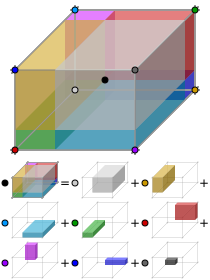
\includegraphics[width=0.5\textwidth]{trilinear.png}
				\caption{Visualization of trilinear interpolation as a~composition of linear interpolations. \textcolor{red}{Image drawn in GeoGebra and inspired by \href{https://commons.wikimedia.org/wiki/File:3D_interpolation2.svg}{a~similar image on Wikipedia} (which looks a~bit worse) -- is credit necessary?}}
				\label{fig:trilin}
			\end{figure}
			
			\textcolor{red}{Maybe a~citation here, although I am not sure it is necessary since it could be considered common knowledge. The~last two equations are my own. Maybe $x_0$, etc. should be explicitly described.}
	\chapter{Track Simulation}
	In order to develop and test the~reconstruction algorithm, electron and positron tracks are simulated inside the~first sector $\mathcal{D}_1$ of our detector (see Section~\ref{sec:coor}) with different initial parameters. Two approaches are currently used to simulate tracks, each of them for different purpose.
	
	The~\textbf{Microscopic Simulation} uses the~\garfieldpp toolkit~\cite{Garfield++}. Within this toolkit, the~\ac{HEED} program~\cite{HEED} is used to simulate the~primary particle and the~class \textit{AvalancheMicroscopic} to simulate the~drift of secondary electrons created by ionization in the~gas. This is the~most precise and time-consuming simulation used; our current goal is to be able to successfully reconstruct its results and determine our best-case energy resolution.
	
	The~\textbf{Runge-Kutta Simulation} uses the~4th order Runge-Kutta numerical integration (\textcolor{red}{add citation for Runge-Kutta}) to simulate the~trajectory of the~primary particle in the~electromagnetic field inside the~detector. It is relatively fast since it does not simulate the~secondary particles. It is used as part of our reconstruction algorithm and for testing some parts of the~reconstruction.
	
	All of these simulations require the~knowledge of the~electromagnetic field inside the~detector. A~uniform electric field of 400~V$\cdot$cm$^{-1}$ is assumed. The~magnetic field was simulated in Maxwell (see Section~\ref{sec:mag}). \textcolor{red}{add citation}
	
	\textcolor{red}{Single track in positive x direction or initial parameter randomization. Importance of gas composition, used gas compositions.}
	
	\section{Microscopic Simulation}
	\label{sec:microsim}
		The~microscopic simulation, the~most detailed simulation used in this work, is performed using the~Garfield++ toolkit~\cite{Garfield++}.
		
		The~electron transport properties are simulated using the~program Magboltz~(\textcolor{red}{Add citation.}). Two different gas mixtures were used: 90\%~Ar~+~10\%~CO$_2$ and 70\%~Ar~+~30\%~CO$_2$. The~second mixture will be used in our detector. The~temperature is set to 20~$^\circ$C, the~pressure is atmospheric.
		
		The~primary track is simulated using the~program~\ac{HEED}~\cite{HEED}, which is an implementation of the~photo-absorption ionization model. This program provides the~parameters of ionizing collisions. \ac{HEED} can also be used to simulate the~transport of delta electrons; we do not account for these in the~current simulation but plan to include them in the~future. The~photons created in the~atomic relaxation cascade (\textcolor{red}{fluorescence reabsorption, ?}) are also not simulated.
		
		Finally, we use the~microscopic tracking provided by the~class \textit{AvalancheMicroscopic} to simulate the~drift of the~ionization electrons. Each electron is followed from collision to collision using the~equation of motion and the~collision rates calculated by Magboltz.
		
		\textcolor{red}{First simulated track in the~$z$ direction should be described in detail here (own subsection?). Figures.}
		
		\textcolor{red}{Add more detailed and better description of HEED, and microscopic tracking (each their own subsection?). Could also mention Monte Carlo (requires gas file generation - Magboltz) and Runge-Kutta simulation implemented in Garfield, why we don't use them (another subsection? rename the~section to \garfieldpp simulation and mention all relevant parts?).}
		
		\begin{figure}[H]
			\centering
			\includegraphics[width=0.3\textwidth]{7030_xz.png}
			\includegraphics[width=0.3\textwidth]{7030_yz.png}
			\includegraphics[width=0.3\textwidth]{7030_xy.png}
			\caption{Example of a~simulated electron track in 70~\%~argon and 30~\%~CO$_2$ atmosphere (on the~left). \textcolor{red}{Swap for better images, better zoom. Explain drift lines, primary particle.}}
			\label{fig:7030sim}
		\end{figure}
		
		\begin{figure}[H]
			\centering
			\includegraphics[width=0.9\textwidth]{diff_comp.png}
			\caption{Comparison of diffusion in a~simulated electron track in 70~\%~argon, 30~\%~CO$_2$ atmosphere and in 90~\%~argon, 10~\%~CO$_2$ atmosphere (on the~right). \textcolor{red}{Swap for better image, better zoom. Or put the~same pictures for both comparisons in one subfigure, etc. Describe better.}}
			\label{fig:diffcomp}
		\end{figure}
	
	\section{Runge-Kutta Simulation}
	\label{sec:rks}
		\textcolor{red}{Trajectory simulation with 4th order Runge-Kutta. Relativistic equation that is numerically integrated by the~algorithm.}	
	\chapter{Track Reconstruction}
\label{sec:track}
	The~first stage of our reconstruction algorithm is the~reconstruction of the track of the~primary particle (electron or positron). The~results of this step are then used to determine the~energy of the~particle (see section~\ref{sec:energy}).
	
	\textbf{First Attempts} at a~track reconstruction were made using the~standard approach. Here we assume we know the~readout coordinates ($x'$,~$y'$,~$t$) exactly (i.e. we neglect the~pads and time bins). In standard \ac{TPC} (with parallel fields) we only need to reconstruct the~$z$~coordinate from drift time using the~known drift velocity.
	
	Reconstruction with the~\textbf{Ionization Electron Map} (from now on referred to as \emph{the~map}) uses simulation of the~drift of the~secondary (ionization) electrons in the~volume of the detector. This simulation can then be used to interpolate the~initial position of the~secondary electrons. First attempts neglect the~pads.
	
	The~\textbf{Discrete Reconstruction} is made using the~map, instead of reconstructing the~exact position of each electron we reconstruct the middle point of each hit pad with time corresponding to the~middle of the~time bin. The number of electrons in each \ac{TPC}~bin (consisting of the~pad and the~time bin) is counted and used as a~charge in the~energy reconstruction.
	
	\textcolor{red}{Reconstruction of one track simulated with microscopic tracking in Garfield++.}
	
	\section{First Attempts}
	\label{sec:trackfirst}
		As the~first step of the~work, we decided to try to reconstruct an~electron track with a~special set of initial parameters. The~origin of the~particle is given by the~origin of our coordinate system. The initial direction is given by the~positive $x$~axis. This means the~magnetic field of our detector is perpendicular to the~momentum of our particle at all times and we can reduce the problem to two dimensional space. We use a~track simulated using the~microscopic simulation (see section~\ref{sec:microsim}) with a~kinetic energy of 8~MeV. The gas composition used in this simulation is 90\%~Ar~+~10\%~CO$_2$.
		
		In this first approach to the~reconstruction of the~track, we decided to use the~common method used in a~standard \ac{TPC}. This will allow us to explore the significance of the~atypical behavior in our \ac{OFTPC}. At the~same time, we consider the~readout to be continuous to further simplify the~problem. In this approximation we reconstruct the~initial position of each ionization electron.
		
		The~reconstruction is then defined by the~following relations between the~coordinates of the~detector space and the~readout space (see section~\ref{sec:coor}):
			\begin{eqnarray}
				x = x',\\
				y = y',\\
				z = v_d t,
			\end{eqnarray}
		where $v_d$ is the~drift velocity of electrons in the~given gas mixture. On a~phenomenological level, this velocity can be considered a~function of the~electric field~$\bm{E}$ and the~magnetic field~$\bm{B}$:
			\begin{equation}
				v_d = v_d(\bm{E},\bm{B}).
			\end{equation}
		\textcolor{red}{Taken from Garfield user manual.} The~Garfield++ toolkit uses this fact to accelerate their drift simulation with non-microscopic approaches. Since we assume uniform electric field in our detector and we want to neglect the~effect of our unusual magnetic field, we consider the~drift velocity to be constant in this scenario. We then approximate this velocity by fitting the dependence $z(t)$ taken from the~simulated ionization electrons.\textcolor{red}{This is in one of the provisional figures. Also this description is not completely accurate, in reality we fit t1:8-y0 with a1*x+a0 and then invert this and use 8-y0 = b1*t1+b0 (old coordinates), b1=1/a1 functions as the drift velocity. Maybe also define this 8-z variable as an alternative to z in the section~\ref{sec:coor} and then use it when correcting this.}
		
		\textcolor{red}{Later, in a commit after this, I plot some residues (provisional figure) which could be useful but for some reason they are residuals from a spline fit of the track?! Probably redo this without the spline fit, just explore the difference in individual points.}
		
		\begin{figure}
			\centering
			\includegraphics[width=0.5\textwidth]{9010_zt.png}
			\caption{Dependence of the~drift time on the~$z$~coordinate in 90~\%~argon and 10~\%~CO$_2$ atmosphere, fitted with a~linear function. The~fitted function gives us the~average drift velocity in the~gas and can be used for rough reconstruction in our \ac{TPC}. \textcolor{red}{Swap for better image with axis labels, etc. Maybe write the~fitted equation.}}
			\label{fig:9010zt}
		\end{figure}
		
		\begin{figure}
			\centering
			\includegraphics[width=0.5\textwidth]{9010_xz.png}
			\caption{First attempt at a~track reconstruction using only the~drift velocity. This approach works well in a~standard \ac{TPC} (\textcolor{red}{ideally cite some source?}). 90~\%~argon and 10~\%~CO$_2$ atmosphere. \textcolor{red}{Swap for better image, correct coordinates.}}
			\label{fig:9010xz}
		\end{figure}
		
		\begin{figure}
			\centering
			\includegraphics[width=0.5\textwidth]{9010_res.png}
			\caption{First attempt at a~track reconstruction using only the~drift velocity, residues. \textcolor{red}{Swap for better image, correct coordinates. What's causing the shift? Explain details.}}
			\label{fig:9010res}
		\end{figure}
	
	\section{Ionization Electron Map}
	\label{sec:map}
		For a~trajectory inside an~\ac{OFTPC}, the~drift of the~secondary (ionization) electrons is significantly affected by its magnetic field. We need to take this into account for accurate reconstruction. In the~first approximation, we assume a~continuous read out (i.e. we neglect pads). We can then reconstruct the~original position of each ionization electron using its readout coordinates. For this purpose, we use the~ionization electron map.
		
		The~ionization electron map is a~mapping between the~detector space and the~readout space. It tells us what readout coordinates $(x',y',t)$ we can expect on average for an~ionization electron created in the~detector coordinates $(x,y,z)$. To get an~approximation of this mapping, we can simulate the~drift of ionization electrons created on a~regular grid inside the~volume of our \ac{OFTPC}. It is also useful to simulate multiple (100 in our case) electrons originating in the same position so we can get a~better approximation of the~average drift. In order to get accurate results, we use the~microscopic simulation of these electrons described in the~section~\ref{sec:microsim}.
		
		Finally, we need to invert the~map to get the~original detector coordinates $(x,y,z)$ for given readout coordinates $(x',y',t)$. \textcolor{red}{Two ways of inverting.}
		
		The~simulation of the~map is a~computationally heavy task. For this reason, we use a~grid MetaCentrum \textcolor{red}{(citation)} to parallelize it. At first, this was done by splitting the~simulated electrons evenly between the~individual jobs. This was used in the~first simulation with only one electron per vertex in the~regular grid with the~spacing of one centimeter. 
		
		Later a~better approach was used accounting for different lengths of the~trajectory of individual electrons. If we index the~electrons in the~order of increasing coordinates $y,x,z$ (\textcolor{red}{picture?}), we can express the~number~$n_l$ of full XY~layers (electrons with the~same $z$~coordinate) of electrons with index less than or equal to $i$
			\begin{equation}
				n_l(i) = \left\lfloor\frac{i}{n_{xy}}\right\rfloor,
			\end{equation}
		where $n_{xy}$ is the~number of electrons in each XY~layer calculated simply by counting the~electrons that satisfy boundary conditions for $x$~and~$y$. \textcolor{red}{These conditions should be mentioned above, sector condition + maximal $x$ value.} The~number of electrons remaining in the~top layer is then
			\begin{equation}
				n_r(i) = i\!\!\!\!\mod n_{xy}.
			\end{equation}
		Finally, we can calculate the sum of the~drift gaps of electrons up to index~$i$
			\begin{equation}
				d_\text{sum} = (z_\text{max}-z_\text{min})n_{xy}n_l-\frac{n_l(n_l-1)}{2}n_{xy}l+n_r(z_\text{max}-z_\text{min}-n_l l).
			\end{equation}
		We then use the~binary search algorithm to look for the~highest value of $i$ that gives us smaller value of this sum than the~fraction $\frac{\text{job id}}{\text{max job id}}$ of the total sum. This way we obtain the~minimal and the~maximal index of electrons simulated in the~given job.
		\textcolor{red}{The spacing $l$ should be probably defined above + picture of the simulating grid (1 layer). zmin zmax also}
		
		\textcolor{red}{Could insert a table here describing all 4 simulations of the map (gas composition, spacing, etc.). Simulation inside one sector (at first double angle). Extra space on sensor. Edge cases not taken into account (TPC wall). Using qsub (not sure if important).}
		
		\textcolor{red}{Explanation of the map, pictures. Simulated on MetaCentrum, workload distribution between multiple jobs. More electrons at one location to get statistics. Two methods of reconstruction using this map. Comparison of 90/10 and 70/30 maps.}
		
		\begin{figure}
			\centering
			\includegraphics[width=0.5\textwidth]{map_9010_gen.png}
			\caption{Example of map generation. \textcolor{red}{Swap for better image, correct coordinates.}}
			\label{fig:map9010gen}
		\end{figure}
		
		\begin{figure}
			\centering
			\includegraphics[width=0.5\textwidth]{9010_reco.png}
			\caption{Example reconstruction with the map. \textcolor{red}{Swap for better image, correct coordinates.}}
			\label{fig:9010reco}
		\end{figure}
		
		\subsection{Gradient Descent Search}
			\label{sec:grad}
			\textcolor{red}{Gradient descent search of a point in the original space that gets mapped to the given point of the readout space (trilinear interpolation).}
		
		\subsection{Interpolating in the Inverse Grid}
			\textcolor{red}{Interpolating between known points in the readout space. Gaussian elimination, multivariate polynomial.}
			
			\begin{figure}
				\centering
				\includegraphics[width=0.8\textwidth]{interpol.png}
				\caption{Selection of the points for interpolation. \textcolor{red}{Create better images, use the explanation interpolation vs extrapolation strange property. Solution~2 probably does not make much sense.}}
				\label{fig:interpol}
			\end{figure}
		
	\section{Discrete Reconstruction}
		\textcolor{red}{Reconstruction with pads and time bins. Maybe testing different pads.}
	\chapter{Energy Reconstruction}
\label{sec:energy}
	The~second stage is the~reconstruction of the~particle's energy using a~fit of its reconstructed track (see Section~\ref{sec:track}). We have tested three ways of reconstructing the~energy. Fitting is done using the~MINUIT algorithm implemented in ROOT~\cite{ROOT}. \textcolor{red}{Cite some CERN article directly on MINUIT, can add a~section.}
	
	The~\textbf{Cubic Spline Fit} is a~tested and later rejected method of energy reconstruction. It uses smoothly connected piecewise cubic polynomials between uniformly spaced nodes. Energy is calculated using the~fit parameters by computing the~radius of curvature in different points of the~fitted curve using the~known magnitude of the~magnetic field perpendicular to the~trajectory. We rejected this method because tuning of the~fit to have a~reasonably stable radius of curvature turned out to be unpractical.
	
	The~\textbf{Circle and Lines Fit} was chosen as an~alternative since this corresponds to the~shape of a~trajectory of a~charged particle crossing a~finite volume with a~homogeneous magnetic field. The~energy of the~particle can be estimated using the~fitted radius and the~magnitude of the~perpendicular magnetic field in the~middle of the~\ac{TPC}.
	
	The~\textbf{Runge-Kutta Fit} uses the~4th order Runge-Kutta numerical integration described in Section~\ref{sec:rks}. Initial parameters of the~track (including the~particle's energy) are optimized so that the~integrated trajectory fits to the~reconstructed one. This fit can also be performed as a~single parameter (i.e., energy) fit if we get the~initial position and orientation of the~particle on the~entrance to the~\ac{TPC} from previous detectors (\ac{Tpx3} and \ac{MWPC}, see Section~\ref{sec:IEAP}).
	
	\begin{figure}
		\centering
		\includegraphics[width=0.5\textwidth]{9010_3d.png}
		\caption{Example of a~fitted reconstructed track. \textcolor{red}{Swap for better image.}}
		\label{fig:90103d}
	\end{figure}
	
	\section{Cubic Spline Fit}
	\label{sec:cspline}
		The~first attempt to get an~early estimate of the~kinetic energy of the~particle uses a~cubic spline fit. We use an~electron track starting in the~origin of our coordinate system with an~initial direction in the~positive $x$~axis. The~ example track is simulated microscopically (see Section~\ref{sec:microsim}) with a~kinetic energy of 8~MeV in a~gas mixture 90\%~Ar~+~10\%~CO$_2$ (the~same track was used in Section~\ref{sec:trackfirst}). \textcolor{red}{This track should probably be described in the~simulation chapter.}
				
		In order to calculate the~spline, we use the~class \textit{TSpline3} from ROOT. This allows us to evaluate the~spline using the~coordinates $(x_n,z_n)$ of each node and the~derivatives $d_1,d_2$ in the~first and the~last node. We can fit these parameters of a~fixed amount of nodes to the~simulated trajectory. We use the~IMPROVE algorithm provided by the~\textit{TMinuit} class in ROOT. This algorithm attempts to find a~better local minimum after converging.
		
		After the~fit, we want to get an~energy estimate. In order to calculate it, we need the~radius of curvature, which we get from the~fitted spline at every point of the~trajectory. The~part of the~spline corresponding to a~given node is defined as
			\begin{equation}
				z(x) = z_n + b \Delta x+c(\Delta x)^2+d(\Delta x)^3,
			\end{equation}
		where $\Delta x = x-x_n$ and $b,c,d$ are coefficients. Using this equation, we derive the~radius of curvature\footnote{For the~general formula see \url{https://en.wikipedia.org/wiki/Curvature\#Graph_of_a_function}} as:
			\begin{equation}
				r(x) = \frac{\left(1+z'^2(x)\right)^\frac{3}{2}}{z''(x)} = \frac{\left(1+\left(b+2c\Delta x+3d(\Delta x)^2\right)^2\right)^\frac{3}{2}}{2c+6d\Delta x}.
			\end{equation}
		Based on the~geometry of the~detector, we can assume the~magnetic field \linebreak$\bm{B}(x,0,z) = (0,B(x,z),0)$ for a~track in the~XZ~plane. Since the~electron is relativistic, the~effect of the~electric field on its trajectory is negligible. The~Lorentz force $F_L$ is then always perpendicular to the~momentum of the~electron and acts as a~centripetal force $F_c$:
			\begin{linenomath}
			\begin{align}
				\bm{F_L} &= \bm{F_c},\\
				\norm{e\bm{v}\times\bm{B}} &= \frac{\gamma m_e v^2}{r},\\
				e c\beta B &= \frac{E_{0e} \beta^2}{r\sqrt{1-\beta^2}},\\
				\sqrt{1-\beta^2} &= \frac{E_{0e} \beta}{ecBr},
			\end{align}
			\end{linenomath}
			\begin{equation}
				\beta^2(x) = \left[1+\left(\frac{E_{0e}}{ecB(x,z(x))r(x)}\right)^2\right]^{-1}, \label{eq:ekin1}
			\end{equation}
		where $e$~is the~elementary charge, $c$~is the~speed of light in vacuum, $m_e$~is the~rest mass of electron, $E_{0e} = m_e c^2$ is the~corresponding energy, $\gamma$~is the~Lorentz factor, $\bm{v}$~is the~velocity of the~electron, and $\beta = \frac{v}{c}$. We can then finally get our estimate of the~kinetic energy for a~given point on the~trajectory as follows:
			\begin{equation}
				\label{eq:ekin2}
				E_\text{kin}(x) = \left(\frac{1}{\sqrt{1-\beta^2(x)}}-1\right)E_{0e}.
			\end{equation}
		We can then average these estimates at multiple points to get one final estimate. This method was later rejected in favor of the~circle and lines fit described in Section~\ref{sec:clines}.
		\textcolor{red}{Add some figures.}
		
		\begin{figure}
			\centering
			\includegraphics[width=0.8\textwidth]{9010_splines.png}
			\caption{First attempt at a~track reconstruction using only the~drift velocity. Spline energy reconstruction attempt. \textcolor{red}{Swap for better image(s) -- subfigure environment, correct coordinates.}}
			\label{fig:9010splines}
		\end{figure}
	
	\section{Circle and Lines Fit}
	\label{sec:clines}
		Another way to estimate the~particle's kinetic energy is to~fit its trajectory with a~circular arc with lines attached smoothly. This shape of trajectory corresponds to a~movement of a~charged particle through a~homogeneous magnetic field perpendicular to the~particle's momentum and limited to a~certain volume. In general, the~shape of such a~trajectory in a~non-perpendicularly oriented field is a~spiral. In our case, this component is negligible since the~field is approximately toroidal and the~particle motion is nearly perpendicular to it. At first, we tested a~2D version of this fit, then we adapted it to 3D.
		
		Our field is not homogeneous, it is therefore not entirely clear what value of magnetic field should be used along with the~fitted radius (using equations~\ref{eq:ekin1} and~\ref{eq:ekin2}) to get the~best estimate for the~kinetic energy. Since we only use this method as the~first iteration of the~particle's energy that we later refine, an~optimal solution of this problem is not required. Instead, we tested two options: taking the~value of the~field in the~middle of the~fitted circular arc and taking the~average field along it. \textcolor{red}{We haven't really tried to plot this for multiple tracks, but these estimates are saved somewhere and could be plotted.}
		
		\subsection{Two-dimensional fit}
			In the~2D case, the~fitted function used for the~electron track\footnote{Electron tracks bend towards negative~$z$, we need to use the~upper part of the~circle} described in Section~\ref{sec:cspline} is defined as follows: \textcolor{red}{Maybe describe this track that we used at the~beginning somewhere earlier (section microscopic simulations \textrightarrow~Testing track?) so that it is easier to refer to it in multiple sections. It is not part of the~early GitHub commits, so maybe it won't be possible to create exact replicas of the~images, but they should be at least very similar.}
				\begin{equation}
					\label{eq:clines2d}
					z(x) = \begin{cases}
								a_1x+b_1 & x<x_1\\
								z_0+\sqrt{r^2-(x-x_0)^2} & x_1\leq x\leq x_2\\
								a_2x+b_2 & x>x_2
						   \end{cases},
				\end{equation}
			where $a_{1,2}$ and $b_{1,2}$ are the~parameters of the~lines, $(x_0,z_0)$ is the~center of the~circle, $r$ is its radius, and $(x_{1,2},z_{1,2})$ are the~coordinates of the~function's nodes. That means we have 9~parameters ($z_{1,2}$ are not used in the~function) along with 2~continuity conditions and 2~smoothness conditions. For the~fit, we use the~coordinates of the~nodes and the~radius of the~circle, which gives us 5~independent parameters (only the~radius has to be larger than half of the~distance between nodes). The~continuity conditions (combined with the~relations for $z_{1,2}$) are as follows:
				\begin{equation}
					\label{eq:ccont}
					z_{1,2} = a_{1,2}x_{1,2}+b_{1,2} = z_0-\sqrt{r^2-(x_{1,2}-x_0)^2}.
				\end{equation}
			The~smoothness conditions are as follows:
				\begin{equation}
					\label{eq:a12}
					a_{1,2} = \frac{x_0-x_{1,2}}{\sqrt{r^2-(x_{1,2}-x_0)^2}}.
				\end{equation}
			Equation~\ref{eq:ccont} gives us the~values of $b_{1,2}$
				\begin{equation}
					\label{eq:b12}
					b_{1,2} = z_{1,2} - a_{1,2} x_{1,2}.
				\end{equation}
			For the~coordinates of the~center of the~circle, we can use the~fact that the~center has to lie on the~axis of its chord. In other words, there is a~value of a~parameter~$t$ such that, using the~parametric equation of the~axis
				\begin{equation}
					\begin{pmatrix} x_0\\ z_0 \end{pmatrix} = \begin{pmatrix} \frac{x_1+x_2}{2}\\ \frac{z_1+z_2}{2} \end{pmatrix} + t \begin{pmatrix} \frac{z_2-z_1}{2}\\ \frac{x_1-x_2}{2} \end{pmatrix}.
				\end{equation}
			At the~same time, the~center has to be in a~distance of $r$ from the~nodes:
				\begin{linenomath}
				\begin{gather}
					(x_1-x_0)^2 + (z_1-z_0)^2 = r^2,\\
					\left(\frac{x_1-x_2}{2}+\frac{z_1-z_2}{2}t\right)^2 + \left(\frac{z_1-z_2}{2}+\frac{x_2-x_1}{2}t\right)^2 = r^2,\\
					\left(\left(\frac{x_2-x_1}{2}\right)^2+\left(\frac{z_2-z_1}{2}\right)^2\right)t^2+\left(\frac{x_2-x_1}{2}\right)^2+\left(\frac{z_2-z_1}{2}\right)^2-r^2=0.
				\end{gather}
				\end{linenomath}
			Since our electron track bends towards negative $z$ and $x_2 > x_1$, we only care about the~solution with $t>0$
				\begin{equation}
					t = \sqrt{\frac{r^2}{\left(\frac{x_2-x_1}{2}\right)^2+\left(\frac{z_2-z_1}{2}\right)^2}-1},
				\end{equation}
				\begin{align}
					x_0 = \frac{x_1+x_2}{2} + \frac{z_2-z_1}{2} \sqrt{\frac{r^2}{\left(\frac{x_2-x_1}{2}\right)^2+\left(\frac{z_2-z_1}{2}\right)^2}-1},\label{eq:x0}\\
					z_0 = \frac{z_1+z_2}{2} - \frac{x_2-x_1}{2} \sqrt{\frac{r^2}{\left(\frac{x_2-x_1}{2}\right)^2+\left(\frac{z_2-z_1}{2}\right)^2}-1}.\label{eq:z0}
				\end{align}
			The~function defined in Equation~\ref{eq:clines2d} along with equations~\ref{eq:a12}, \ref{eq:b12}, \ref{eq:x0} and~\ref{eq:z0} derived using the~continuity and smoothness conditions (combined with the~relations for $z_{1,2}$) fully define our fitted function with parameters $r,x_{1,2},z_{1,2}$. \textcolor{red}{Some pictures of the~fit on the~tested track. Results of the~fit. Again, the~actual fit uses 8-z. Use GeoGebra schematics to generate a~picture of 2D geometry.}
			
			\begin{figure}
				\centering
				\includegraphics[width=0.8\textwidth]{9010_circle2D.png}
				\caption{First attempt at a~track reconstruction using only the~drift velocity. Circle and Lines Fit in 2D. \textcolor{red}{Swap for better image, correct coordinates.}}
				\label{fig:9010circle2D}
			\end{figure}
		
		\subsection{Three-dimensional fit}
			\textcolor{red}{Explain the geometry and least square method used for the~3D fit. Tested on a~Runge-Kutta sample, and with microscopic tracks + map simulation.}
			
			In three dimensions, the~shape of a~trajectory of a~charged particle in a~uniform magnetic field is a~cylindrical helix. since we assume that the field is approximately perpendicular to the~particle's momentum at all times, we will further approximate the~trajectory with a~circular arc (with lines attached smoothly).
			
			We assume that the~initial position $\mathbf{X}_0 = (x_0,y_0,z_0)$ and direction $\theta,\varphi$ (\textcolor{red}{spherical angles as in Section~\ref{sec:coor}}) are known, since this information will be provided by \ac{Tpx3} and \ac{MWPC} layers. \textcolor{red}{We could further refine it at the~end of the current algorithm with some kind of global fit (all detector layers).} The fit then has four free parameters (\textcolor{red}{figure}):
				\begin{itemize}[nosep]
					\item the length of the first line $l$ (as measured from the initial position),
					\item the radius of the circular arc $r$,
					\item the central angle of the arc $\phi_\text{max} \in [0,2\pi]$,
					\item the direction of the curvature given by the angle $\alpha \in [0,2\pi]$ (right-handed with respect to the particle direction, $\alpha = 0$ if the particle curves towards negative~$z$ in a~plane given by~$\hat{z}$ and the direction vector).
				\end{itemize}
			Using these parameters, we can derive a parametrization of the~whole curve. Let $\mathbf{v}$ be the initial unit direction vector, i.e., using the spherical angles
				\begin{equation}
					\mathbf{v} = (\cos\varphi\cos\theta, \,\sin\varphi\cos\theta, \,\sin\theta)^\mathrm{T},
				\end{equation}
			then we can parameterize the first line as follows:
				\begin{equation}
					\mathbf{X}_\text{L1}(t) = \mathbf{X}_0 + t\mathbf{v} \quad t\in[0,l].
				\end{equation}
			This gives us the starting point of the~arc
				\begin{equation}
					\mathbf{X}_1 = \mathbf{X}_\text{L1}(l) = \mathbf{X}_0 + l\mathbf{v}.
				\end{equation}
			The vector $\mathbf{n}\perp\mathbf{c}_1$ that lies in the~plane of curvature and points from $\mathbf{X}_1$ to the~center of curvature can be calculated using a composition of rotations. First, we rotate $\mathbf{v}$ to point in the~$\mathbf{\hat{x}}$ direction, the normal for $\alpha = 0$ than points in the $-\mathbf{\hat{z}}$ direction, we apply the $\alpha$ rotation and reverse the rotations into the~$\mathbf{\hat{x}}$ direction:
				\begin{equation}
					\begin{aligned}
						\mathbf{c}_1 &= R_z(\varphi)R_y(-\theta)R_x(\alpha)R_y\left(\frac{\pi}{2}\right)R_y(\theta)R_z(-\varphi)\mathbf{v},\\
						&= R_z(\varphi)R_y(-\theta)R_x(\alpha)(-\mathbf{\hat{z}}),\\
						&= \scalebox{0.95}{$
								\begin{pmatrix}
									\cos\varphi & -\sin\varphi & 0\\
									\sin\varphi & \cos\varphi & 0\\
									0 & 0 & 1
								\end{pmatrix}
								\begin{pmatrix}
									\cos\theta & 0 & -\sin\theta\\
									0 & 1 & 0\\
									\sin\theta & 0 & \cos\theta
								\end{pmatrix}
								\begin{pmatrix}
									1 & 0 & 0\\
									0 & \cos\alpha & -\sin\alpha\\
									0 & \sin\alpha & \cos\alpha
								\end{pmatrix}
								\begin{pmatrix}
									0\\ 0\\ -1
								\end{pmatrix}
							$},\\
						&= 	\begin{pmatrix}
								-\sin\alpha\sin\varphi+\cos\alpha\cos\varphi\sin\theta\\
								\phantom{-}\sin\alpha\cos\varphi+\cos\alpha\sin\varphi\sin\theta\\
								-\cos\alpha\cos\theta
							\end{pmatrix}.
					\end{aligned}
				\end{equation}
			\textcolor{red}{Seems like in this part of the~code $\theta$ is actually taken from the~pole.} Similarly by rotating $\mathbf{\hat{y}}$, we can get the~normal vector $\mathbf{n}=\mathbf{v}\cross\mathbf{c}_1$ perpendicular to the~plane of the~trajectory:
				\begin{equation}
					\mathbf{n} = R_z(\varphi)R_y(-\theta)R_x(\alpha)\mathbf{\hat{y}}=
									\begin{pmatrix}
										-\cos\alpha\sin\varphi-\sin\alpha\cos\varphi\sin\theta\\
										\phantom{-}\cos\alpha\cos\varphi-\sin\alpha\sin\varphi\sin\theta\\
										\sin\alpha\cos\theta
									\end{pmatrix}.
				\end{equation}
			This allows us to express the coordinates of the~center of the~circular arc:
				\begin{equation}
					\mathbf{C} = \mathbf{X}_1+r\mathbf{c}_1.
				\end{equation}
			We can then get the parametrization and the endpoint of the~circular arc using Rodrigues' rotation formula:
				\begin{gather}
					\begin{aligned}
						\mathbf{c}_2 &= \mathbf{c}_1\cos\phi_\text{max} + (\mathbf{n}\cross\mathbf{c}_1)\sin\phi_\text{max} + \mathbf{n}(\mathbf{n}\cdot\mathbf{c}_1)(1-\cos\phi_\text{max}),\\
						&= \mathbf{c}_1\cos\phi_\text{max} - \mathbf{v}\sin\phi_\text{max},
					\end{aligned}\\
					\mathbf{X}_C(\phi) = \mathbf{C} - r(\mathbf{c}_1\cos\phi - \mathbf{v}\sin\phi) \quad \phi\in[0,\phi_\text{max}],\\
					\mathbf{X}_2 = \mathbf{X}_C(\phi_\text{max}) = \mathbf{C} - r\mathbf{c}_2,
				\end{gather}
			and if we define the~direction vector of the~second line, we also get its parametrization
				\begin{gather}
					\mathbf{w} = \mathbf{v}\cos\phi_\text{max} + (\mathbf{n}\cross\mathbf{v})\sin\phi_\text{max} = \mathbf{v}\cos\phi_\text{max} + \mathbf{c}_1\sin\phi_\text{max},\\
					\mathbf{X}_\text{L2}(s) = \mathbf{X}_2 + s\mathbf{w} \quad s\in[0,\infty).
				\end{gather}
				
			The fit is performed as a~(weighted) least square minimization (\textcolor{red}{MIGRAD ROOT}), therefore we need to derive the~distance of any point~$\mathbf{P}$ to the~fitted curve. For the first line, we simply compute the parameter value of the~closest point on the line:
				\begin{align}
					t_P &= \mathbf{v}\cdot(\mathbf{P}-\mathbf{X}_1),\\
					d_{P1} &= \norm{\mathbf{P}-\mathbf{X}_\text{L1}(t_P)}.
				\end{align}
			If the parameter value is outside of its bounds defined above, we take the boundary value instead. The distance to the~second line is computed likewise. For the~circular arc, we find the closest point by projecting the~center connecting line onto the~arc plane:
				\begin{gather}
					\mathbf{X}_{PC} = \mathbf{X}_C + r\frac{(\mathbf{P-\mathbf{X}_C})-(\mathbf{n}\cdot(\mathbf{P-\mathbf{X}_C}))\mathbf{n}}{\norm{(\mathbf{P-\mathbf{X}_C})-(\mathbf{n}\cdot(\mathbf{P-\mathbf{X}_C}))\mathbf{n}}},\\
					d_{PC} = \norm{\mathbf{P}-\mathbf{X}_{PC}}
				\end{gather}
			\textcolor{red}{Potential problem in the implementation -- might not be correctly handling $\phi$ out of bounds, the distance could be sometimes underestimated because of this.} The~shortest distance out of $d_{P1},d_{PC},d_{P2}$ is then taken as the distance to the~curve. \textcolor{red}{When calculating energy with the average field, only the arc is considered. Middle field in the current implementation taken in the middle~$x$ plane (intersection with the curve). TVirtualFitter+MIGRAD.}
			
			\begin{figure}
				\centering
				\includegraphics[width=0.8\textwidth]{circlefit.png}
				\caption{Circle and Lines Fit 3D geometry. \textcolor{red}{Swap for better image.}}
				\label{fig:circlefit}
			\end{figure}
	
	\section{Runge-Kutta Fit}
		\textcolor{red}{Single parameter fit with 4th order Runge-Kutta simulated track. Future testing with microscopic simulations and map simulation. Derivation of the~geometry (least squares).}
	
	\chapwithtoc{Conclusion}
	We have developed and implemented several methods for the reconstruction of electron and positron trajectories inside the Orthogonal Fields Time Projection Chambers (\acp{OFTPC}) that will be used in the X17 project at the \acf{IEAPCTU} to confirm or disprove the ATOMKI anomaly~\cite{atomki_be}. We tested these methods on simulated tracks and made a~preliminary estimate of the achievable energy resolution.
	
	We used the \garfieldpp toolkit~\cite{Garfield++} for simulations in combination with the ROOT~framework~\cite{ROOT} for data analysis and visualization. Some of our more demanding simulations were run on the MetaCentrum grid~\cite{metacentrum}. The main method of track simulation was the microscopic simulation (provided by the \texttt{Avalanche\-Microscopic} class), which follows ionization electrons from collision to collision.
	
	\subsubsection*{Track Reconstruction}
		The inhomogeneous magnetic field created by permanent magnets is perpendicular to the electric field of the chambers and has a~significant effect on the drift of ionization electrons (as demonstrated in \cref{sec:rasd}). For this reason, we created the ionization electron map, i.e., a~mapping from the detector space~$\mathcal{D}$ (coordinates $(x,y,z)$), where the initial positions of ionization electrons lie, to the readout space~$\mathcal{R}$ (coordinates $(x',y',t)$), where their endpoints on the readout plane lie. The map was simulated using the microscopic simulation. One hundred electrons with low initial velocity were simulated for each point on a~Cartesian grid to get their mean readout coordinates and their covariance. Two gas mixtures 90:10 and 70:30 Ar:CO$_2$ were compared. In the former, the drift velocity is significantly higher, leading to an increased effect of the magnetic field and larger diffusion (see, for example, \cref{fig:map_yx_bot}).
		
		To use the map in reconstruction, we have to invert it. We implemented two methods -- a~gradient descent algorithm that finds a~minimum in the trilinearly interpolated map, and a~polynomial interpolation on the inverse grid in the readout space (where we know the inverse from the simulation). Both methods reach almost identical results for the testing track, while the latter is much faster, does not require optimization of parameters, and can be accelerated by precalculating the interpolation coefficients in the future if needed. The reconstruction was shown to be accurate with less than \qty{2}{\mm} \acs{FWHM}, although a~slight shift in the $z$\nobreakdash-coordinate was detected when accounting for different initial velocities of the ionization electrons (see \cref{fig:9010_map_res,fig:7030_map_res}).
		
		The discrete reconstruction takes into account the anode segmentation into pads and the finite size of the time bins. It neglects the gaps between the pads and assumes an ideal readout of charge, counting each individual electron hitting the pad. Charge multiplication in the triple-\ac{GEM} stack used in the \ac{OFTPC} is not taken into account. For each pad/time-bin combination, we use the map inversion to reconstruct its center. Reconstruction of detector coordinates corresponding to electrons hitting pad 12 near the magnet pole (\cref{fig:pad_reco,fig:pad_reco_old}) shows that interpolation on the inverse grid behaves pathologically for large distortions, unlike the much slower gradient descent algorithm, likely because of large coefficients of the quadratic and cubic terms.
		
	\subsubsection*{Energy Reconstruction}
		To reconstruct the energy of a~particle in a~\ac{OFTPC}, we assess its curvature in the inhomogeneous magnetic field. Preliminary tests were done using tracks reconstructed with the map with no discretization. At first, we tested a~cubic spline fit, where the radius of curvature can be determined analytically. This approach turned out to be unpractical because of relatively low speed, and the necessity to create the energy estimate from the radius and magnetic field at different points on the track (see \cref{fig:spline}).
		
		Another tested approach (at first as a~2D version without pads, later in 3D with pads) was the fit with a~circular arc with smoothly attached lines, which is the shape of trajectory of a~particle crossing a~finite volume with homogeneous magnetic field oriented perpendicularly to the particle's velocity vector. This way we get a~single reconstructed radius of curvature, however, since the magnetic field varies greatly along the track inside the \ac{OFTPC} volume, it is not clear, which value of magnetic field to use to calculate the energy. Two simple estimates were implemented:
		\begin{enumerate}[nosep]
			\item using the value at the point, where the track crosses the middle $x$\nobreakdash-coordinate and
			\item using the average value along the circular arc in the fit,
		\end{enumerate}
		in both cases, only the component perpendicular to the plane of the fit is considered. The three-dimensional version of the fit has four free parameters (radius, length of the first line, length of the circular arc, and rotation angle around the first line). In order for the fit to converge correctly in all cases, the parameter bounds have to be set carefully. Disallowing pathological values that are not expected for any real track may cause the MIGRAD algorithm to converge at the bound. The fit was successfully tested on a~sample of Runge-Kutta tracks described in \cref{sec:rktest}; the results in \cref{fig:cfit_rk} show that the average field estimate systematically underestimates the energy of the track, but its \acs{FWHM} is much smaller than that of the middle field estimate.
		
		The best developed method was the Runge-Kutta fit. In a~simplified model, we assume that the previous layers of detectors will provide us with exact initial position and direction of the particle, when entering the \ac{OFTPC}. We can then use 4th\nobreakdash-order Runge-Kutta numerical integration to simulate such a~trajectory for different energies. In order to speed up the fit and ensure convergence of the fit, we use a~corrected estimate from the circle-and-lines fit with average field as a~starting point. We tested this method on a~grid-like sample of microscopic tracks, described in \cref{sec:microgrid}, fitting tracks reconstructed with the discrete map inversion. As shown in \cref{fig:rk_dE}, we can reach energy resolution (\acs{FWHM}) \qty{1.56}{\percent} for electrons (which curve away from the readout, enabling charge spreading across multiple channels) and \qty{1.95}{\percent} for positrons without correcting systematic errors dependent on the track parameters, assuming an ideal charge readout with no noise and no amplification.
		
		The code used in this thesis, and in related work, is available publicly at \url{https://github.com/Vavrikus/x17-utef}.
	\section*{Future}
	\addcontentsline{toc}{section}{Future}
		In order to develop a~functioning algorithm for the real detector, there are still many things left to account for. Here are some examples of what steps can or will be taken next.
		
	\subsubsection*{Simulations}
		There are several important factors that need to be considered when simulating the detector response:
		\begin{itemize}
			\item Charge multiplication on the triple-\ac{GEM} and limited efficiency of the readout. In some cases, the spreading of charge between multiple pads during multiplication might have a~positive effect on the resolution.
			\item Noise in the data. We are currently tuning an algorithm for track de-noising using a~convolutional neural network~\cite{Gajdoš_2025}.
			\item Delta electrons released by the particle.
			\item Electron attachment and Penning transfer in the gas mixture. Influence of even small amounts of other gases needs to be considered.
			\item Energy loss of the primary electrons and positrons.
			\item Better simulation of magnetic and electric fields; so far we have been assuming that the electric field is homogeneous. A~simulation of the triple~\ac{GEM} could be included, but some simplifications would be necessary, since the microscopic simulation needed for such a~structure is extremely time-consuming.
			\item Account for the triggering in \ac{MWPC} and \acf{TPX3} detector layers. While a~small uncertainty of the drift time measurement may not be relevant for the energy reconstruction in a~standard \ac{TPC} with a~homogeneous magnetic field, a~shift of the entire trajectory along the $z$\nobreakdash-coordinate in our detector changes the magnetic field along the track, and therefore the reconstructed energy.
			\item An optimization study of the pad layout is possible with the current algorithm.
		\end{itemize}
		It might be also useful to use a~faster simulation method for more robust reconstruction testing. Currently, a~simple Monte Carlo simulation, using the covariance matrices from the map simulation, is implemented and can be used along with \ac{HEED} to simulate tracks similar to the microscopic ones. The microscopic simulation is very time-consuming, we have already spent \num{25165.6} CPU days during the simulation of the grid-like testing sample, and partly during the map simulation.
		
	\subsubsection*{Experimental calibration}
		To achieve the best results, the reconstruction needs to be calibrated using measurements from the real detector. This includes:
		\begin{itemize}
			\item measurement of the magnetic field of the permanent magnets,
			\item reconstruction of straight tracks from laser or muons, and
			\item reconstruction of electrons with known energy distribution, if possible.
		\end{itemize}
		
	\subsubsection*{Reconstruction algorithm}
		Several tweaks are being considered to improve the reconstruction algorithm in the future:
		\begin{itemize}
			\item Optimization --- multiple Runge-Kutta fits could be run with gradually decreasing step size.
			\item Estimation of errors using the error of the fit.
			\item Accounting for the variable initial velocity of ionization electrons produced by the incident particle. The current map uses initial energy \qty{0.1}{\eV}, which led to systematic errors in the $z$\nobreakdash-coordinate reconstruction, as shown in \cref{fig:7030_map_res}. Another map could be simulated with different initial direction and energy distributions, tracking the ionization electrons only until they slow down to the mean drift velocity, and using the already simulated map from there. Alternatively, we could correct the reconstructed $z$\nobreakdash-coordinate based on the reconstructed curve of the track using some rough estimate obtained from a~grid-like simulation of microscopic tracks.
			\item If a~speed optimization is needed, a~discrete pad map could be calculated ahead of time, instead of repeated calculation during the reconstruction. At this moment, the most computationally expensive part of the reconstruction is the individual fits. The slower gradient descent map inversion technique may be used to avoid issues with the interpolation on the inverse grid (shown in \cref{fig:pad_reco}).
			\item At the end of the fitting procedure, we could refine the origin and the initial direction of the track obtained from the previous detector layers with some kind of global fit.
			\item Using maximum likelihood for the energy fit, instead of the least squares method. Currently, in the discrete map inversion reconstruction, we reconstruct the center of each hit pad and time bin. However, due to the drift distortion, this may not correspond to the most likely, or even the average position to be hit by an ionization electron.
			
			In theory, we could by taking into account the whole map $\mathcal{M}$ (including the covariance matrices, describing the multivariate normal distribution that describes each map point well according to our preliminary tests), we could make an "inverse map" from $\mathcal{R}$ to distributions on $\mathcal{D}$. We could achieve this by taking the normalized probability density of an electron with initial coordinates $(x,y,z)$ having readout coordinates $(x',y',t)$. If we fix $(x',y',t)$, we get an unnormalized probability density $f(x,y,z) = \mathcal{M}_{(x,y,z)}(x',y',t)$ (assuming that all initial coordinates are a~priori equally likely). This could potentially improve the discrete reconstruction if we take the mean value of this probability density across the pad and time bin
			\begin{equation}
				f_\text{pad, bin}(x,y,z) = \frac{1}{A_\text{pad} \Delta t_\text{bin}} \int_\text{pad, bin} \mathcal{M}_{(x,y,z)}(x',y',t) 	\text{d}x'\text{d}y'\text{d}t
			\end{equation}
			and using it for a~likelihood fit instead of using least squares. This still assumes that all initial coordinates are equally likely which is clearly not the case for a~primary particle track. In the future, we could even use the fast track simulation with the map (it should be possible to make around 1000 tracks or more per minute per core with current settings), create a~big set of tracks with reasonable parameters and use these to get an approximation of the probability distribution of the detector response. Some approximations would be necessary when interpreting the data to decrease the degrees of freedom of this distribution (we would have to pick a~set of parameters and assume that some of them are independent). This could give us an idea about the best achievable resolution (how significantly will the detector response differ for a~given change in energy). If the difference is significant, we could try to further improve the likelihood fit.
		\end{itemize}
	
	%%% Bibliography
	\include{bibliography}
	
	%%% Figures used in the thesis (consider if this is needed)
	\listoffigures
	
	%%% Tables used in the thesis (consider if this is needed)
	%%% In mathematical theses, it could be better to move the list of tables to the beginning of the thesis.
	\listoftables
	
	%%% Abbreviations used in the thesis, if any, including their explanation
	%%% In mathematical theses, it could be better to move the list of abbreviations to the beginning of the thesis.
	
\chapwithtoc{List of Abbreviations}
\begin{acronym}
	\acro{GEM}{Gas Electron Multiplier}
	\acro{HEED}{High Energy Electro-Dynamics}
	\acro{IEAPCTU}[IEAP~CTU]{Institute of Experimental and Applied Physics, Czech Technical University in Prague}
	\acro{IPC}{Internal Pair Creation}
	%\acro{IPCC}{Internal Pair Conversion Correlation}
	\acro{EPC}{External Pair Creation}
	\acro{Micromegas}{MICRO-MEsh GAseous Structure}
	\acro{MWPC}{Multi-Wire Proportional Chamber}
	\acro{OFTPC}{Orthogonal Fields \ac{TPC}}
	\acro{RK4}{Runge-Kutta 4th order}
	\acro{TPC}{Time Projection Chamber}
	\acro{ToA}{time\protect\nobreakdash-of\protect\nobreakdash-arrival}
	\acro{ToT}{time\protect\nobreakdash-over\protect\nobreakdash-threshold}
	\acro{Tpx3}{Timepix~3}
\end{acronym}
	
	%%% Attachments to the bachelor thesis, if any. Each attachment must be
	%%% referred to at least once from the text of the thesis. Attachments
	%%% are numbered.
	%%%
	%%% The printed version should preferably contain attachments, which can be
	%%% read (additional tables and charts, supplementary text, examples of
	%%% program output, etc.). The electronic version is more suited for attachments
	%%% which will likely be used in an electronic form rather than read (program
	%%% source code, data files, interactive charts, etc.). Electronic attachments
	%%% should be uploaded to SIS and optionally also included in the thesis on a~CD/DVD.
	%%% Allowed file formats are specified in provision of the rector no. 72/2017.
	% \appendix
	%\chapter{Attachments}
	
	%\section{First Attachment}
	
	% \openright
\end{document}